%%%%%%%%%%%%%%%%%%%%% chapter.tex %%%%%%%%%%%%%%%%%%%%%%%%%%%%%%%%%
%
% sample chapter
%
% Use this file as a template for your own input.
%
%%%%%%%%%%%%%%%%%%%%%%%% Springer-Verlag %%%%%%%%%%%%%%%%%%%%%%%%%%

%\motto{Use the template \emph{chapter.tex} to style the various elements of your chapter content.}
\chapter{An Overview of LTE Advanced}
\label{overview-lte} % Always give a unique label
% use \chaptermark{}
% to alter or adjust the chapter heading in the running head

%\abstract*{Each chapter should be preceded by an abstract (10--15 lines long) that summarizes the content. The abstract will appear \textit{online} at \url{www.SpringerLink.com} and be available with unrestricted access. This allows unregistered users to read the abstract as a teaser for the complete chapter. As a general rule the abstracts will not appear in the printed version of your book unless it is the style of your particular book or that of the series to which your book belongs.
%Please use the 'starred' version of the new Springer \texttt{abstract} command for typesetting the text of the online abstracts (cf. source file of this chapter template \texttt{abstract}) and include them with the source files of your manuscript. Use the plain \texttt{abstract} command if the abstract is also to appear in the printed version of the book.}

\abstract{This chapter provides a high-level overview of LTE-Advanced (LTE-A) networks and associated technologies to form a basis for discussion of the co-existence issues that exist for unlicensed LTE and Wi-Fi. Understanding the underlying architecture and protocols employed in LTE-A networks will provide readers a comparative framework to grasp how, and at what levels, LTE and Wi-Fi networks may interact and interfere with each other, and form a greater understanding of the challenges to be address in designing coexistence mechanisms. Specifically, this chapter will overview the LTE-A network, its capabilities and protocols, with specific emphasis on the physical layer and medium access sub-layers to illuminate specific sources of co-existence issues. Proposed changes which may be included in future LTE releases are discussed in the context of LTE/Wi-Fi coexistence.}


\section{System Overview}
\label{sys-overview}
The enhancements to the Long Term Evolution/System Architecture Evolution (LTE-SAE) to meet the requirements set out for fourth generation (4G) cellular networks are collectively known as LTE-Advanced, and were formalized in 3GPP TR 36.913, releases 10 through 13 \cite{tr36913}.  LTE itself was a logical evolution from the GSM/EDGE and UMTS/GPRS/HSPA technologies used in previous generations to meet the increasing demands for higher data rates and improved quality of service. LTE meets these demands at the access level through improved spectral efficiency, using OFMDA and SC-FDMA for downlink and uplink, respectively, and improved mobility support and cell edge data rates through enhanced adaptive modulation and bandwidth selection and downlink spatial multiplexing support. To support these gains beyond the access layer, LTE transitioned to an all IP packet switched core network with the introduction of the evolved packet core, and a flattened network architecture of enhanced base stations called evolved NodeB's (eNB) which are interconnected via high-speed.  Combined, this allowed LTE networks to significantly increase user data rates and reduce control and user plane latency and connection set-up and handover times.  

\subsection{Network Architecture}
\label{net-arch}
The requirements to provide high data rates while supporting high-speed mobility requires the ability to set up and tear down user connections and manage inter-cell handoffs with as little latency as possible.  The hierarchical structure consisting of base stations or NodeBs connected to a central controller which had been used in past cellular networks requires additional hops in both data transmissions and hand off negotiation which can introduce significant delay as the controller manages handoffs betweens several pairs of base stations, as well as all other voice and data traffic.  For many increasingly ubiquitous end-user applications, such as online gaming and video conferencing, the additional latency in connection set up and handover can impair the user quality of experience.  

To meet these requirements, LTE adopted the flat architecture shown in Fig. \ref{figs:LTE-A-Network} and migrated the functions of radio network, medium access control, handoff request, negotiation, and managements, as well as some other truly local functions, to the eNBs themselves and provided high-speed, low latency, connections between the eNBs in a mesh configuration \cite{tr36300}. 
%TODO:Consider better figure?
\begin{figure}[!ht]
	\centering
	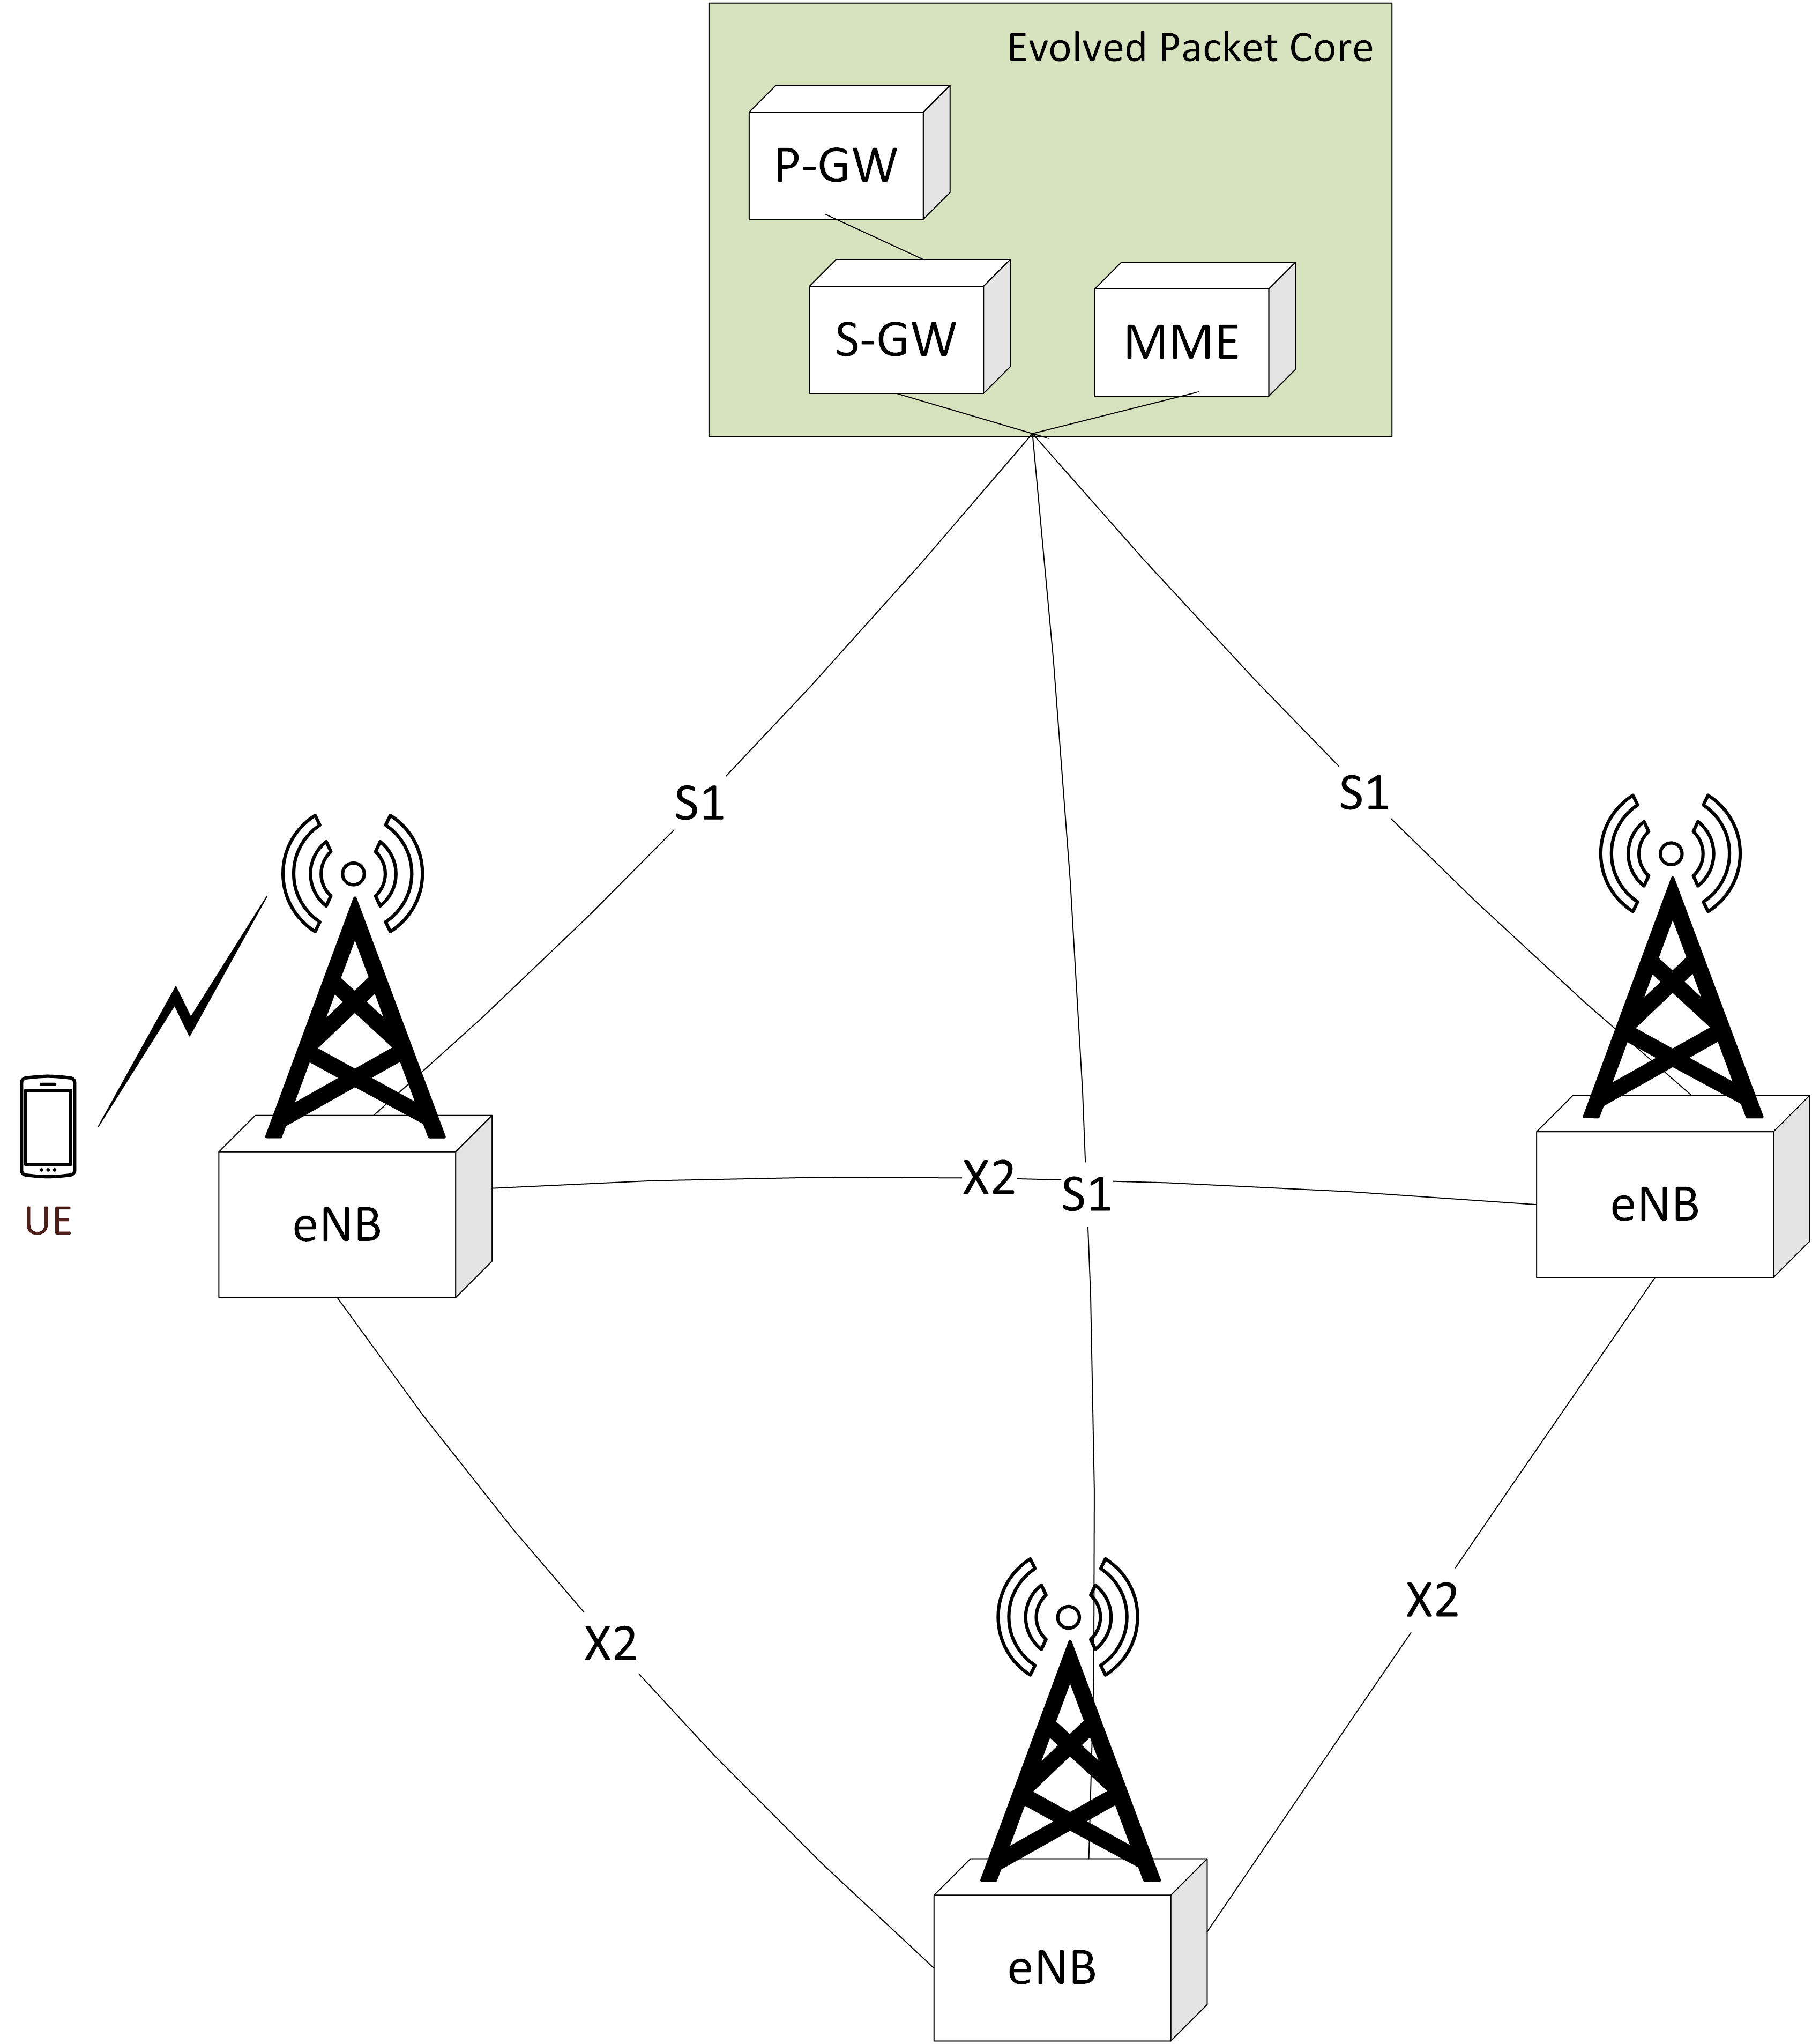
\includegraphics[width=2.5in]{figures3/lteAnet}
	\caption{Basic structure of LTE-A cellular network.}
	\label{figs:LTE-A-Network}
\end{figure}
The global functions and connections to external networks are handled at the evolved packet core (EPC in the the figure). The mobile management entity (MME) handles authentication, authorization and accounting functions, among others.  The packet data network gateway (P-GW) and serving gateway (S-GW) handle user data packet forwarding, filtering, and usage tracking, as well as acting as a mobility anchor for inter-eNB and inter-RAT handovers.  The functional split between the various components of the network is shown in further detail in Fig. \ref{figs:funcSplit}.

%TODO: Figure MUST be changed as it is taken from 3GPP doc for reference/placeholder only
\begin{figure}[!ht]
	\centering
	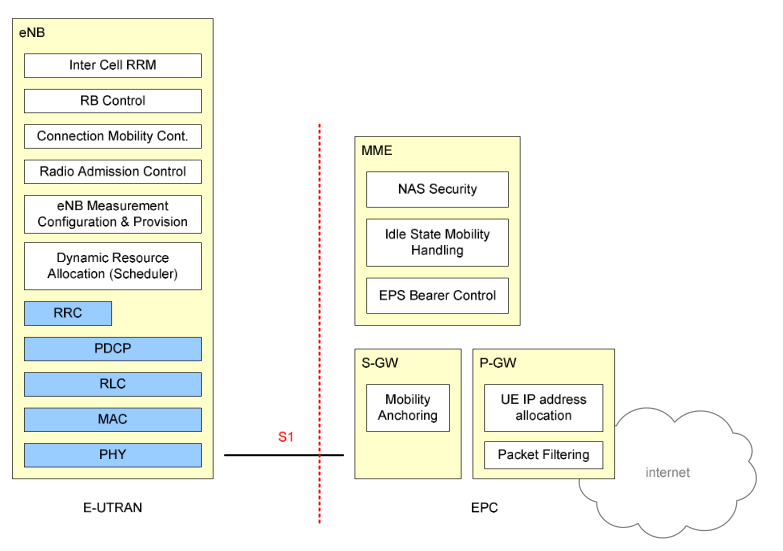
\includegraphics[width=4.25in]{figures3/functionalsplit}
	\caption{Functional split between eNodeB and evolved packet core.}
	\label{figs:funcSplit}
\end{figure}

The distributed radio network and medium access control allows eNBs to quickly adapt to changing radio medium condition and user scheduling based on local information.  The low-latency X2 interface connections between eNBs allows for fast user handover, including forwarding of queued data for seamless user experience.  Additionally, with direct connections between neighbouring cells, this architecture facilitates more effective multi-point transmission and reception coordination and inter-cell interference and load management, independent of conditions in other areas of the network.  

\subsection{Capabilities and Features}

While the gains made by LTE were significant, they fell short of the requirements set out for 4G networks by the International Telecommunications Union, specifically in the case of peak data rates, spectral efficiency, and cell edge performance \cite{itu-advanced}. Some important ITU requirements and achieved performance levels for LTE and LTE-A are highlighted in Table \ref{perf-table}PLACEHOLDER:

%TODO: verify the contents/details of this table and expand if possibe
\begin{table}
	\caption{ITU-A Requirements for 4G vs. LTE/LTE-A Achievements \cite{lte-3gpp}\cite{lteA-3gpp}\cite{itu-advanced}\cite{abdullah}}
	\label{perf-table}      
	\begin{tabular}{p{4.8cm}p{2.4cm}p{2.4cm}p{2.4cm}}
		\hline\noalign{\smallskip}
		Description/Requirements & ITU-A & LTE & LTE-A   \\
		\noalign{\smallskip}\svhline\noalign{\smallskip}
		DL peak spectral efficiency (bps/Hz) &  15   & 15  & 30 \\
		UL peak spectral efficiency (bps/Hz)& 6.75  & 3.75  & 15 \\
		Min. cell edge spectral \\ \hspace{0.8em} efficiency (bps/Hz) & 0.04 & 0.024 & 0.04 \\
		DL Peak data rates (Mbps) & 1000$^1$  & 300 & 1000 \\
		UL Peak data rates (Mbps) & 1000$^1$  & 75 & 500 \\
		Scalable bandwidth up to (MHz) & 40 & 20  & 100$^2$ \\
		
		\noalign{\smallskip}\hline\noalign{\smallskip}
	\end{tabular}
	$^1$ For low mobility with requirement of min. 100 Mbps for speeds of up to 350 km/h. 	 \\
	$^2$ With carrier aggregation of up to five carrier components.
\end{table}

Among other innovations, in order to meet these requirements, LTE-A extends bandwidth scalability in LTE by supporting carrier aggregation to increase bandwidth. Backwards compatibility is maintained by using bandwidths for each carrier component which match those used in LTE.  Discontiguous aggregation is supported to ensure a higher bandwidth is available for providers who cannot support it in contiguous spectrum allotments, opening the door to LTE in shared bands.  LTE-A also expands MIMO/spatial multiplexing support up to 8x8 for DL and 4x4 for UL, adds coordinated multi-point operation and relay nodes to increase spectral efficiency and cell edge data rates, and improves heterogeneous network planning with the enhancement of support for small cells and relay nodes to increase area coverage with reduced power requirements.

\section{Channel Access Mechanisms}
\label{channel-access}
Like other cellular access technologies, LTE-A has been designed for use on dedicated licensed spectrum allocations where there is, generally, no need to contend for channel access.  While interference, fading, and path loss can corrupt LTE transmissions, and recovery and retransmission functions are necessary, in general a centrally controlled and tightly scheduled channel access mechanism is able to guarantee service levels required by all uplink and downlink traffic \cite{tr36300}.  Channel access is achieved through frequency division multiple access (FDMA) and either time or frequency division duplexing.  Orthogonal frequency division (OFDMA) is used in the downlink to allow the eNB to efficiently schedule transmissions for many users in the same transmission time interval.  Single carrier frequency division (SC-FDMA) is used in the uplink to reduce the power consumption requirements of battery dependent user equipment (UE) to communicate with the eNB.  Further, coordinated multipoint (CoMP) is supported by allowing UEs to be configured to process channel state information from multiple eNBs, and both single-user and multi-user MIMO are supported in multiple configurations to achieve transmit diversity or multi-layer transmissions with beamforming possible in both horizontal and vertical dimensions.

The basic structure of the protocol stack used in LTE networks to facilitate channel access is shown in Fig. \ref{figs:stack} \cite{tr36201}.
%TODO: Figure MUST be changed as it is taken from 3GPP doc for reference/placeholder only
\begin{figure}[!ht]
	\centering
	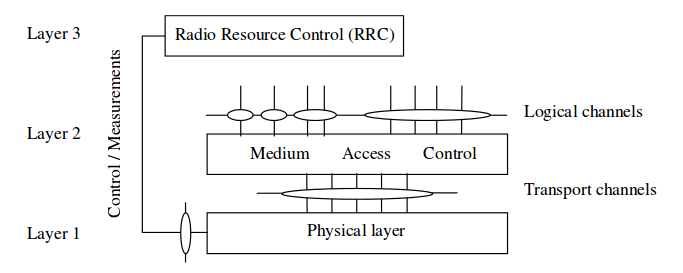
\includegraphics[width=3.5in]{figures3/protocolStack}
	\caption{E-UTRA radio interface protocol architecture.}
	\label{figs:stack}
\end{figure}
UL and DL transmissions are divided amongst several physical channels, according to the type of transmission, i.e. traffic or control information, and the type of transmission, i.e broadcast or unicast and scheduled or random access. The information bearing physical channels are mapped by the PHY layer into transport channels supplied to the MAC sublayer, which in turn remaps these into logical channels provided to the higher layers. 

\subsection{LTE-A Physical Layer}
\label{lte-phy}
The LTE PHY layer is designed to be both widely adoptable as well spectrally and power efficient.  In the DL, OFDMA is used to schedule many signals in the same transmission time interval and achieve a high spectral efficiency, however, the very high peak to average power ratio makes this multiple access strategy unattractive in the UL for battery dependent devices \cite{tr36201}\cite{tr36211}.  SC-FDMA is used in the UL to maintain a satisfactory spectral efficiency while significantly improving power efficiency and battery life. An example carrier allocation multiple access strategy for both OFDMA and SC-FDMA is shown in Fig. \ref{lte:of-sc-fdma}.

%%TODO: Make new figure, this is copied as a placeholder
\begin{figure}[!ht] 
	\centering
	\subfloat[OFMDA used in downlink.]{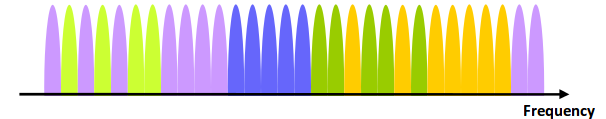
\includegraphics[width=4in]{figures3/lte-ofdma}%
		\label{ofdma}}
	\\
	\subfloat[SC-FDMA used in uplink.]{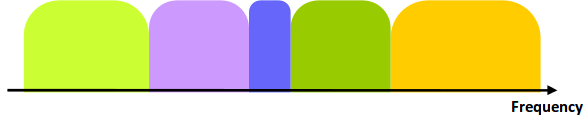
\includegraphics[width=4in]{figures3/lte-scdma}%
		\label{sc-fdma}}
	\caption{PLACEHOLDER: Multiple access strategies used in LTE for uplink and downlink.}
	\label{lte:of-sc-fdma}
\end{figure} 

To support the widest range of devices and spectrum allocations available to carriers, variable transmission bandwidth, and both TDD and FDD are supported in both UL and DL. Additionally, the PHY layer provides forward error correction and automatic repeat requests, modulation/demodulation of physical channels, mapping and rate matching of physical channels to transport channels, frequency and time synchronization, and MIMO antenna processing, including transmit diversity and beamforming.  A variety of modulation schemes are supported depending on channel conditions, distance from receiver, and power requirements (up to 256 QAM in the downlink), and up to 16 transmit antennas, supporting both single and multi-user MIMO to achieve transmit diversity gains or up to 8 streams, with 3D beamforming.


All transmission are organized into frames comprised of ten 1 ms subframes, each of which is formed from two equal length slots \cite{tr36211}. The basic LTE frame structure is shown in Fig. \ref{lte:frame}.
%TODO:Make new figure, this figure is a placeholder only
\begin{figure}[!t]
	\centering
	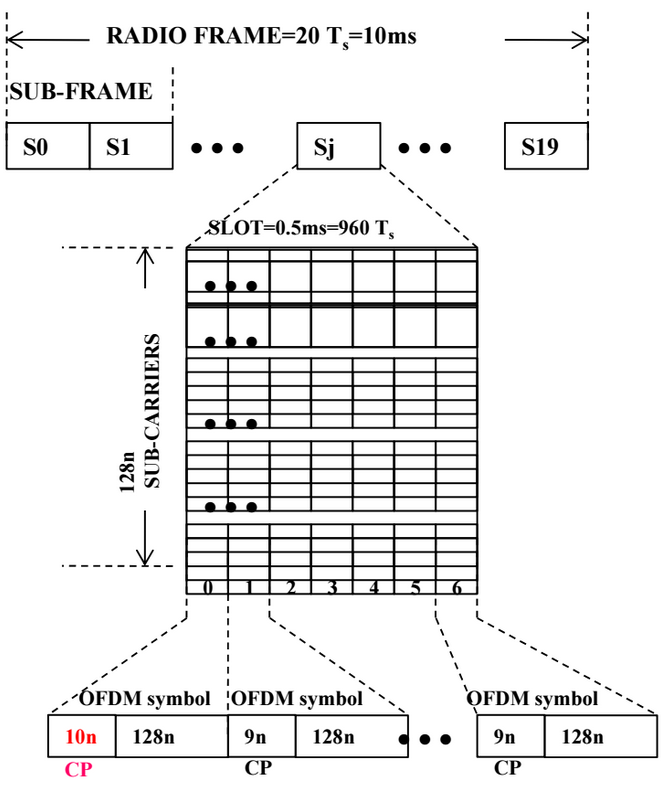
\includegraphics[width=3in]{figures3/lte-frame}
	\caption{PLACEHOLDER: LTE frame and resource block}
	\label{lte:frame}
\end{figure}
The minimum unit which can be allocated to a physical channel or user is the physical resource block (PRB).  A PRB a time and frequency mapping formed of either twelve sub-carriers of bandwidth 15 kHz or 24 sub-carriers of bandwidth 7.5kHz, allocated for one 0.5 ms slot, where between 6 and 10 PRBs will be allocated to achieve bandwidths between 1.4 and 20 MHz (though the occupied bandwidth will be smaller, 1.08 to 18 MHz).  Higher bandwidths are achieved through carrier aggregation in the same slot, either contiguous or not.  

To support both TDD and FDD, two distinct frame structures are defined, as well as a third frame structure specifically for license assisted access (LAA-LTE) in the unlicensed bands.  All three have the same basic structure, with the differences being in how transmission are scheduled.  For FDD, both half and full duplex are supported and 10 subframes are available for both UL and DL, with transmissions separated in frequency only, for full duplex, or time and frequency for half duplex.  For TDD, the frame is organized into two 5 ms half-frames, with several UL/DL configurations and switching patterns supported.  As of Release 13, the special frame structure defined for LAA-LTE reserves all 10 subframed for DL, with transmission occupying one or more consecutive subframes, starting anywhere within the first subframe.


\subsection{LTE-A Medium Access Control}
\label{lte-mac}
Medium access is tightly controlled and scheduled in both UL and DL in LTE-A, with the eNB controlling the time and frequency resource block assignment for all but random access channels (used for UE connection requests and some other procedures) \cite{tr36321}.  Distinct MAC sublayers for the UE and the eNB are defined, as well as several configurations for UE, depending on the specific functions implemented, such as dual connectivity (similar to carrier aggregation but across small and macro cells) or sidelink for UE to UE communication. The basic structure of the MAC sublayer is shown in Fig. \ref{figs:lte-mac}.
%TODO: Decide if a figure is really needed here, and if so make a new one as this one cannot be used in publication
\begin{figure}[!ht]
	\centering
	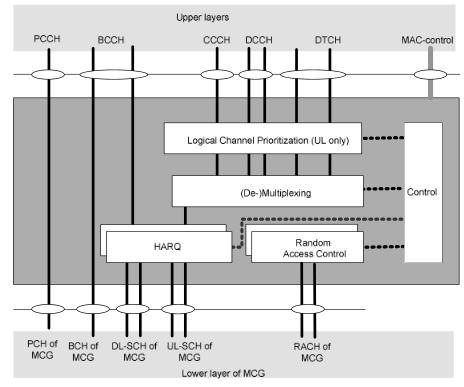
\includegraphics[width=3.5in]{figures3/lteAmac}	\caption{PLACEHOLDER: LTE MAC sublayer detail.}
	\label{figs:lte-mac}
\end{figure}
The MAC sublayer facilitates reliable data transfer through radio resource allocation and the mapping and multiplexing between transport channels and one or more logical channels.  Further, the MAC sublayer handles HARQ signaling, channel prioritization with dynamic scheduling, random access control, data transfer, and scheduling information reporting and requests.  

The specific implementation of these, and other layer 2 functions such as radio link control, are quite complex and beyond the scope of this brief, however the underlying design paradigm is that global of knowledge facilitating tight control over medium usage. The MAC sublayer in the eNB is aware of the channel conditions for each UE to be scheduled in both the UL and DL, and the UE adheres to the schedule of time and frequency provided by the eNB.  PRBs are assigned to UL and DL transmissions to achieve the greatest advantage from local channel conditions. Little consideration of inter-user or inter-carrier interference is necessary, due to the dedicated frequency bands and orthogonal carriers discussed in Sec. \ref{lte-phy}.  

%Consider section change to sources of coexistence issues
\section {Changes Expected for Future Releases}
\label{fut-chnge}
%Am considering dropping this section as it may not be interesting in the context of the rest of the book, would be either rather short OR very technical, and possible a section (such as in my 610 paper) detailing how the preceding sections contribute to potential sources of coexistence issues
LTE-A brings cellular networks into the realm of 4G, as defined by \cite{itu-advanced}.  As far as LTE-A has taken us, it will not be enough for fifth generation networks which are expected to support use cases ranging from smart cities and Internet of Things devices to  self-driving vehicles and industrial automation with \emph{gigabyte} per second, high speed mobile broadband \cite{itu-2020}.  In The ITU has set targets for 5G around peak and average data rates, spectral and energy efficiency, mobility, capacity and density which current wireless networks are incapable of achieving.  

In order to move towards 5G networks, 3GPP has numerous study items underway and planned for future releases, to meet the ITU requirements in \cite{itu-2020}.  These include significant enhancements to inter- and intra-band carrier aggregation and licenses-assisted access to ISM bands, TV white space, and other under-utilized spectrum resources, as well as multi-carrier enhancements and improved CoMP and device to device communications \cite{lteA-gantt}.  Wireless network virtualization and hardware resource sharing, cloud-based radio access networks, and new system architectures are under consideration to support the requirements around energy efficiency and and low-latency communications, among others.  Additionally, the possibility of moving to an entirely new radio and medium access protocols is also under consideration, which would not be hindered by the need to be backwards compatible, and move forward with only the necessity of meeting the ITU 5G requirements.  


%%%%%%%%%%%%%%%%%%%%%%%% referenc.tex %%%%%%%%%%%%%%%%%%%%%%%%%%%%%%
% sample references
% %
% Use this file as a template for your own input.
%
%%%%%%%%%%%%%%%%%%%%%%%% Springer-Verlag %%%%%%%%%%%%%%%%%%%%%%%%%%

\begin{thebibliography}{99.}%
	\bibitem{tr36913}{3GPP}, ``Requirements for further advancements for Evolved Universal Terrestrial Radio Access (E-UTRA) (LTE-Advanced),'' \emph{{3GPP TR 36.913 version 13.0.0 Release 10}}, 2011.
	\bibitem{lte-3gpp} 3GPP, ``{LTE},'' Whitepaper, ND. Accessed: June 21, 2016 [Online]. Available: \url{{www.3gpp.org/technologies/keywords-acronyms/98-lte}}
	\bibitem{itu-advanced}{ITU}, ``Requirements related to technical performance for IMT-Advanced radio interface(s),'' \emph{Rep. ITU-R M.2134}, 2008. 
	\bibitem{tr25.913}{3GPP}, ``Requirements for Evolved UTRA (E-UTRA) and Evolved UTRAN (E-UTRAN),'' \emph{{3GPP TR 25.913 version 8.0.0 Release 8}}, 2009.
	\bibitem{tr36321}{3GPP}, ``Evolved Universal Terrestrial Radio Access (E-UTRA); Medium Access Control (MAC) protocol specification,'' \emph{{3GPP TR 36.321 version 13.1.0 Release 13}}, 2016.
	\bibitem{tr36201}{3GPP}, ``Evolved Universal Terrestrial Radio Access (E-UTRA); LTE physical layer; General description,'' \emph{{3GPP TR 36.201 version 13.1.0 Release 13}}, 2016.	
\end{thebibliography}
